\chapter{Entropy, Equilibrium, and the Maximum-Entropy Problem}

This lecture begins as a deliberate reset. We go back to the basic objects of statistical mechanics: a discrete set of states, a probability distribution over them, the corresponding energies, and the entropy of that distribution. But the reset is not merely definitional. Very quickly the lecture turns those definitions into a picture of equilibrium, then into the thermodynamic laws, then into a derivation of the direction of heat flow, and finally into the real mathematical problem of the subject: which probability distribution maximizes entropy when the total probability and the average energy are fixed?

\paragraph{Credit.} These notes follow Leonard Susskind's lecture, with lecture curation by LazyingArt LLC and Video2Book.

\section{Entropy, Probability, and Average Energy}

We begin exactly as the lecture does. Suppose somebody simply hands us a probability distribution \(P(i)\) over a discrete set of states \(i\). We are not yet asking where the distribution came from; that question is postponed. For the moment we only assume that the states are discrete enough that they can be counted.

Each state has a probability \(P(i)\), and each state has an energy \(E(i)\). The first relation is just normalization,
\begin{equation}
\sum_i P(i)=1,
\end{equation}
and the second is the definition of the average energy,
\begin{equation}
\sum_i P(i)E(i)=\langle E\rangle.
\end{equation}
On the board this appears in precisely that notation, with \(E(i)\) rather than the cleaner \(E_i\). Later, when the algebra becomes heavier, it will be more convenient to write \(E_i\), but at the opening of the lecture it is helpful to keep the board notation in view.

Entropy is then defined by
\begin{equation}
S=-\sum_i P(i)\log P(i).
\end{equation}
The lecture pauses over the minus sign. At first sight the formula looks negative, but it is not. Since \(0<P(i)\le 1\), each \(\log P(i)\) is nonpositive, and therefore every term \(-P(i)\log P(i)\) is nonnegative. So the entropy is a positive quantity.

The opening board layout captures all of this at once: the entropy functional at upper left, the two constraints at upper right, and beneath them a family of distributions drawn against energy.

\begin{figure}[htbp]
\centering

\includegraphics[width=0.88\textwidth]{lecture_03_figure_02.png}
\caption{Entropy, the normalization and average-energy constraints, and a family of equilibrium probability distributions at increasing average energy.}
\end{figure}

Already the lecture is telling us that we should not think only of one distribution. We should think of a whole family of them.

\section{Equilibrium as a Family of Distributions}

Susskind immediately recalls the picture from the previous lecture: a one-parameter family of probability distributions, plotted against the energy of the state and parameterized by the average energy. As the distribution broadens and drifts toward larger \(E\), the average energy increases.

There is also a distinguished endpoint of the family. At the minimum possible energy, the probability distribution is concentrated entirely at the ground state. Then there is no uncertainty left about which state the system occupies, and the entropy is exactly zero.

The lecture leans on a qualitative interpretation of entropy here. Entropy is, roughly speaking, a measure of how many states matter underneath the distribution. A very narrow distribution singles out very few important states; a broader one spreads its weight over many of them. Thus, for the equilibrium families we care about, larger average energy comes together with larger entropy.

It is useful to record that as the working assumption
\begin{equation}
\frac{dS}{d\langle E\rangle}>0,
\end{equation}
but only for the equilibrium family under discussion. This is not a theorem about arbitrary invented distributions.

The board sketch is qualitative, and a clean redraw should stay qualitative as well.

\begin{figure}[htbp]
\centering
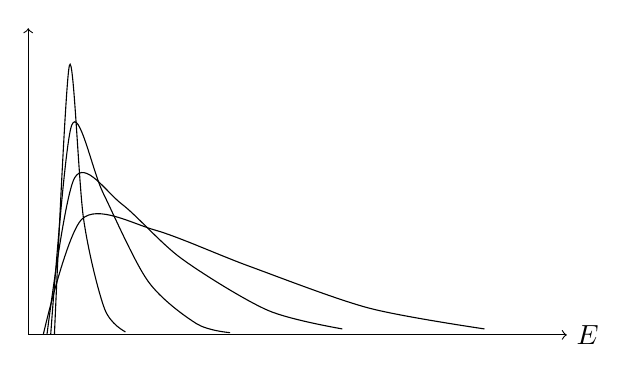
\begin{tikzpicture}[scale=0.95]
\draw[->] (0,0) -- (7.2,0) node[right] {$E$};
\draw[->] (0,0) -- (0,4.1);
\draw[smooth] plot coordinates {(0.35,0) (0.55,3.6) (0.74,1.55) (1.02,0.35) (1.30,0.04)};
\draw[smooth] plot coordinates {(0.30,0) (0.58,2.8) (1.00,1.9) (1.60,0.72) (2.25,0.15) (2.70,0.03)};
\draw[smooth] plot coordinates {(0.25,0) (0.62,2.1) (1.25,1.75) (2.05,1.02) (3.20,0.33) (4.20,0.08)};
\draw[smooth] plot coordinates {(0.20,0) (0.72,1.55) (1.70,1.40) (2.95,0.92) (4.55,0.36) (6.10,0.08)};
\end{tikzpicture}
\caption{Interpretive redraw of the equilibrium family. The board makes the qualitative point: as the average energy increases, the distribution broadens and extends toward larger \(E\).}
\end{figure}

\subsection{Question \& Answer}

Could a distribution move to the right and at the same time get narrower? Certainly. One can invent such a family without difficulty. The lecture says so explicitly. The point is not that probability theory forbids it. The point is that the thermal-equilibrium distributions we are after are not like that. For those distributions, broadening with increasing average energy is exactly the right picture.

\section{Broadening, Coarse-Graining, and the Thermodynamic Laws}

From this picture the lecture pivots to thermodynamics. Thermal equilibrium is characterized by the probability distribution of the states. Of course one may characterize equilibrium by a temperature, but one may also characterize it by an average energy. If a box of gas is in thermal equilibrium, then, in the lecture's phrase, whatever was going to happen has finished happening. Microscopically the molecules still move, but macroscopically the system is quiescent, mixed up, and no longer evolving in any dramatic way.

In that state heat tends not to flow, because all parts of the system are in equilibrium with each other.

Now the laws of thermodynamics can be read in the language of probability distributions. The first law is simply energy conservation. The second law says that entropy increases. But what does that mean in the present setting? It means that when a system starts away from equilibrium and is allowed to come to equilibrium, the probability distribution generally broadens.

This is where the lecture introduces coarse-graining. To coarse-grain is, in effect, to be a little careless about the exact microscopic information. Once we lose track of details, the distribution tends to spread rather than sharpen. A narrowing distribution would mean that somehow we had learned more and more about an enormous complicated system without actually measuring it. That is not the natural direction of things. The natural direction is that we lose track, the distribution broadens, and entropy grows.

The zeroth law is then presented in a modernized way. Historically it entered thermodynamics axiomatically, but here the lecture treats it as illuminated by the first and second laws together with the definition of temperature already introduced. There exists a notion of temperature such that energy flows from higher temperature to lower temperature, and in equilibrium all parts of the system have the same temperature.

The lecture now asks the natural question: does the earlier definition of temperature really know which way heat flows? Let us test it.

\section{Temperature and the Direction of Heat Flow}

Take a system made of two connected parts, \(A\) and \(B\), able to exchange energy. Assume, just to fix conventions, that
\begin{equation}
T_B>T_A.
\end{equation}
If the opposite inequality held, we would merely interchange the labels.

The first law gives
\begin{equation}
dE_A+dE_B=0,
\end{equation}
because the total energy of the combined system is conserved.

The second law gives
\begin{equation}
dS_A+dS_B\ge 0,
\end{equation}
with equality only in special cases. Generically the total entropy increases.

Now use the earlier definition of temperature,
\begin{equation}
dE=T\,dS.
\end{equation}
Applied separately to the two subsystems,
\begin{equation}
dE_A=T_A\,dS_A,
\qquad
dE_B=T_B\,dS_B.
\end{equation}
Substituting these into energy conservation, we obtain
\begin{equation}
T_A\,dS_A+T_B\,dS_B=0.
\end{equation}
Solve for \(dS_B\):
\begin{equation}
dS_B=-\frac{T_A}{T_B}\,dS_A.
\end{equation}
Now eliminate \(dS_B\) from the entropy inequality:
\begin{align}
dS_A+dS_B &\ge 0, \\
dS_A-\frac{T_A}{T_B}dS_A &\ge 0, \\
\left(1-\frac{T_A}{T_B}\right)dS_A &\ge 0.
\end{align}
For the moment we assume temperatures are positive. Multiplying by \(T_B>0\) gives
\begin{equation}
(T_B-T_A)dS_A\ge 0.
\end{equation}
But \(T_B-T_A>0\) by assumption. Therefore
\begin{equation}
dS_A>0.
\end{equation}
Multiplying once more by \(T_A\), we get
\begin{equation}
dE_A=T_A\,dS_A>0.
\end{equation}
So subsystem \(A\) gains energy, and therefore subsystem \(B\) loses it. Energy flows from \(B\) to \(A\), that is, from the hotter subsystem to the colder one.

This is the point of the calculation. Starting from energy conservation, entropy increase, and the definition \(dE=T\,dS\), we recover the physical meaning of temperature: it determines the direction of heat flow. In the lecture, when Susskind says ``heat'' here, he simply means energy transfer.

The flow continues until the temperatures become equal. When
\begin{equation}
T_A=T_B,
\end{equation}
there is no preferred direction for further transfer, and thermal equilibrium is established. The transitive part of the zeroth law then becomes obvious: if \(A\) is in equilibrium with \(B\), and \(B\) with \(C\), then all three have the same temperature.

\subsection{Question \& Answer}

Does this derivation assume that \(A\) and \(B\) are each individually in equilibrium? Yes, it does. The very use of \(T_A\) and \(T_B\) presupposes that each subsystem is internally equilibrated enough for a temperature to be assigned to it. If that is not true, then one must subdivide further. The same reasoning is then applied to smaller pieces until the local equilibrium assumption becomes appropriate.

\section{What a State Means}

Only after the heat-flow argument is finished does the lecture stop and ask a more basic question: what is a state?

A state, we are told, means as much as one can possibly know about the system if one were infinitely powerful, subject always to the actual laws of physics. That last clause matters. In classical mechanics one is tempted to say that a state of a gas is the complete list of positions and momenta of all the molecules. As a first picture, that is the right thing to have in mind. But quantum mechanics places limits on what can be known simultaneously, and in the quantum description the state counting for a finite box becomes discrete.

So there are really two layers here. The conceptual layer is invariant: a state is the most refined description allowed by the theory. The technical layer depends on context: in a quantum treatment we sum over discrete states, while in a classical limit those sums are replaced by integrals. The lecture emphasizes that passing carefully from the quantum description to the classical one is subtle, but the broad statement is correct.

\subsection{Question \& Answer}

Should we literally think of the state of a gas as the position and momentum of every molecule? In the classical picture, yes, that is the right image. But one should immediately add the lecture's caveat: quantum mechanics changes what ``as much as can be known'' means. The useful definition is therefore the more general one. A state is not simply a list of classical variables; it is the finest specification of the system permitted by the laws of physics.

\section{Replicas, Occupation Numbers, and Maximum Entropy}

Now we come to what the lecture itself calls the hard question. Once equilibrium has been reached, what is the probability distribution \(P(i)\) over the microstates?

To get a handle on that question, it is useful to imagine that the system of interest is not isolated but in contact with a very large reservoir, a heat bath, with which it can exchange energy. Because the bath is enormous, a small flow of energy into or out of the subsystem barely changes the bath's temperature.

A particularly convenient model of the heat bath is then introduced. Instead of an amorphous reservoir, imagine a very large number \(N\) of identical copies of the subsystem, all weakly connected so that energy can flow among them. One of them is the subsystem we care about; the rest collectively play the role of the bath. This is not merely a trick. In many physical situations a large system really can be regarded as built from many similar smaller subsystems.

\paragraph{From Counting to Probability.}

Each replica is in some state \(i\). Let \(n_i\) denote the occupation number, the number of replicas found in the \(i\)-th state. The board at this point shows an energy axis with many discrete level marks and writes the basic identification very clearly:

\begin{figure}[htbp]
\centering

\includegraphics[width=0.82\textwidth]{lecture_03_figure_03.png}
\caption{Probability as the occupation fraction \(P(i)=n_i/N\).}
\end{figure}

Thus
\begin{equation}
P(i)=\frac{n_i}{N}.
\end{equation}
In words: the probability that a given subsystem is in state \(i\) is simply the fraction of the replicas that are in that state.

From here on it is convenient to write the state energies as \(E_i\). The occupation numbers satisfy two constraints. First, the total number of replicas is fixed:
\begin{equation}
\sum_i n_i = N.
\end{equation}
Second, the total energy is fixed. If \(E\) denotes the average energy per subsystem, then
\begin{equation}
\sum_i n_i E_i = N E.
\end{equation}
Using \(n_i=NP_i\), these become
\begin{equation}
\sum_i P_i=1,
\qquad
\sum_i P_iE_i=E.
\end{equation}
So the familiar constraints on probabilities are just the occupation-number constraints rewritten per subsystem.

\paragraph{Multiplicity.}

The next question is purely combinatorial: for a given set of occupation numbers \(\{n_i\}\), how many ways are there to distribute the \(N\) replicas among the states so as to realize exactly that set?

The answer is
\begin{equation}
C=\frac{N!}{\prod_i n_i!},
\end{equation}
and the lecture suggests calling this \(C\), for the combinatorial factor. If some occupation numbers are zero, nothing blows up, because
\begin{equation}
0!=1.
\end{equation}
So unoccupied states simply contribute a factor of one to the denominator.

The lecture pauses long enough to check the formula against simple cases. If all \(N\) replicas lie in one state and all other occupation numbers vanish, then
\begin{equation}
C=\frac{N!}{N!}=1,
\end{equation}
as it should: there is only one way to put everything in one cup. If three replicas occupy three different states, then
\begin{equation}
C=\frac{3!}{1!\,1!\,1!}=6.
\end{equation}
Again that is exactly right.

Why do we care about \(C\)? Because of a symmetry argument. If all microscopic redistributions compatible with the setup are treated symmetrically, then the most probable macroscopic occupation pattern is the one realized in the largest number of ways. So the statistical-mechanical problem becomes: maximize \(C\), but maximize it subject to the two constraints above.

\paragraph{Stirling's approximation.}

To do that we need an approximation for large factorials. The lecture takes time to derive the simplified form of Stirling's approximation that is sufficient for this problem.

Start from
\begin{equation}
\log N! = \sum_{x=1}^{N}\log x.
\end{equation}
For large \(N\), replace the sum by an integral:
\begin{align}
\log N! &\approx \int_1^N \log x\,dx \\
&= \left[x\log x-x\right]_1^N \\
&= N\log N-N+1.
\end{align}
The additive constant is negligible on the scale of \(N\), and the lecture keeps only the leading terms:
\begin{equation}
\log N!\approx N\log N-N.
\end{equation}
Exponentiating,
\begin{equation}
N!\approx N^N e^{-N}.
\end{equation}
The familiar \(\sqrt{2\pi N}\) factor, together with other subleading corrections, is deliberately omitted. For the present argument only the leading exponential behavior matters.

One may ask whether Stirling's approximation is justified in the denominator as well as the numerator. The lecture's answer is that, in the large-\(N\) regime of interest, the relevant occupation numbers scale proportionally with \(N\). As the total number of replicas grows, the typical \(n_i\) grow with it, so the same approximation applies to the important denominator terms.

\paragraph{From multiplicity to entropy.}

Apply the approximation upstairs and downstairs:
\begin{equation}
C\approx
\frac{N^N e^{-N}}{\prod_i n_i^{\,n_i}e^{-n_i}}.
\end{equation}
Because \(\sum_i n_i=N\), the exponential factors cancel, leaving
\begin{equation}
C\approx \frac{N^N}{\prod_i n_i^{\,n_i}}.
\end{equation}
Now take the logarithm:
\begin{equation}
\log C = N\log N-\sum_i n_i\log n_i.
\end{equation}
Substitute \(n_i=NP_i\):
\begin{align}
\log C
&= N\log N-\sum_i NP_i\log(NP_i) \\
&= N\log N-N\sum_i P_i\bigl(\log N+\log P_i\bigr) \\
&= N\log N-N\log N\sum_i P_i-N\sum_i P_i\log P_i.
\end{align}
Using \(\sum_i P_i=1\), the \(N\log N\) terms cancel, and we find
\begin{equation}
\log C=-N\sum_i P_i\log P_i = NS.
\end{equation}
This is the decisive turn of the lecture. Maximizing the number of ways of rearranging the replicas is the same as maximizing the entropy. Therefore the most probable occupation-number distribution is obtained by solving
\begin{equation}
\text{maximize } S(P_i)=-\sum_i P_i\log P_i
\end{equation}
subject to
\begin{equation}
\sum_i P_i=1,
\qquad
\sum_i P_iE_i=E.
\end{equation}
That is the statistical-mechanical rule.

\subsection{Question \& Answer}

By symmetry, shouldn't all the occupation numbers simply be equal? They would, if there were no energy constraint. Without constraints, the arithmetic does push toward uniformity. But the states have different energies, and the condition
\begin{equation}
\sum_i P_iE_i=E
\end{equation}
breaks that symmetry. The asymmetry does not come from nowhere; it comes from the fact that not all states cost the same energy.

\section{Lagrange Multipliers and the Problem Left for Next Time}

The lecture does not solve the entropy-maximization problem yet. Instead it spends the rest of the time introducing the tool needed to solve it: Lagrange multipliers.

Without constraints, the rule for extremizing a function \(F(x_1,x_2,\dots)\) is familiar:
\begin{equation}
\frac{\partial F}{\partial x_i}=0
\qquad
\text{for all } i.
\end{equation}
But here the extremization is constrained. One wants to maximize or minimize a function while demanding that some other function vanish:
\begin{equation}
G(x_1,x_2,\dots)=0.
\end{equation}

The lecture first explains the geometry. In two variables, the level curves of \(F\) are like contours on a map, while \(G=0\) is a constraint curve cutting across them. The constrained extremum lies where a level curve of \(F\) is tangent to the constraint curve.

\begin{figure}[htbp]
\centering
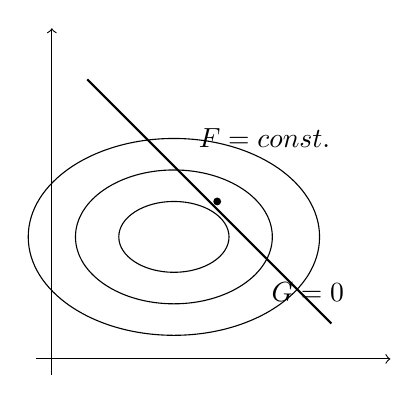
\begin{tikzpicture}[scale=1.0]
\draw[->] (-0.2,0) -- (4.3,0);
\draw[->] (0,-0.2) -- (0,4.2);
\draw (1.55,1.55) ellipse (0.70 and 0.45);
\draw (1.55,1.55) ellipse (1.25 and 0.85);
\draw (1.55,1.55) ellipse (1.85 and 1.25);
\draw[thick] (0.45,3.55) -- (3.55,0.45);
\fill (2.10,2.00) circle (0.05);
\node at (3.25,0.85) {$G=0$};
\node at (2.70,2.80) {$F=\text{const.}$};
\end{tikzpicture}
\caption{Interpretive contour sketch for one constrained extremization problem. The constrained extremum occurs at tangency.}
\end{figure}

The analytic trick is the devilishly clever part. Instead of extremizing \(F\) subject to \(G=0\), define
\begin{equation}
F' = F+\lambda G,
\end{equation}
where \(\lambda\) is a new unknown, the Lagrange multiplier. One then extremizes \(F'\) as though there were no constraint, and afterwards imposes \(G=0\) to determine \(\lambda\).

The lecture works through a simple example:
\begin{equation}
F=\frac{x^2+y^2}{2},
\qquad
G=x+y-1.
\end{equation}
So
\begin{equation}
F'=\frac{x^2+y^2}{2}+\lambda(x+y-1).
\end{equation}
Now set the derivatives of \(F'\) to zero:
\begin{equation}
\frac{\partial F'}{\partial x}=x+\lambda=0,
\qquad
\frac{\partial F'}{\partial y}=y+\lambda=0.
\end{equation}
Hence
\begin{equation}
x=y=-\lambda.
\end{equation}
The remaining equation is simply the original constraint,
\begin{equation}
x+y=1.
\end{equation}
Therefore
\begin{equation}
-2\lambda=1,
\qquad
\lambda=-\frac12,
\end{equation}
and so
\begin{equation}
x=y=\frac12.
\end{equation}
That is the point on the line \(x+y=1\) where \((x^2+y^2)/2\) is minimized.

With several constraints one proceeds in the same way:
\begin{equation}
F'=F+\lambda_1 G_1+\lambda_2 G_2+\cdots,
\end{equation}
and then solves the stationarity equations together with
\begin{equation}
G_1=0,\qquad G_2=0,\qquad \dots
\end{equation}

Now the real statistical-mechanical problem can be written in precisely that language. We want to maximize
\begin{equation}
S(\{P_i\})=-\sum_i P_i\log P_i
\end{equation}
subject to the two constraints
\begin{equation}
G_1=\sum_i P_i-1=0,
\qquad
G_2=\sum_i P_iE_i-E=0.
\end{equation}
That is the mathematics problem the lecture leaves for next time. Once those equations are solved, the equilibrium probability distribution is known.

The lecture also makes a broader point here. At this stage we are not really doing the theory of gases or superconductors in any detailed sense. We are doing probability theory: maximizing an entropy, or equivalently a multiplicity, subject to constraints. The same mathematics appears in many contexts. Statistical mechanics is the physical arena in which those constrained probability problems become unavoidable.

And there is one more hint before the lecture ends: temperature itself will turn out to be a Lagrange multiplier.

\section{Summary}

What began as a recap has turned into a precise program. We started from a probability distribution over states, wrote its average energy and entropy, and pictured a family of equilibrium distributions whose entropy grows with energy. We then translated the thermodynamic laws into the language of distributions and used \(dE=T\,dS\) to show that energy flows from hotter to colder subsystems until their temperatures equalize. After that the lecture changed point of view: from one system to many replicas, from probabilities to occupation numbers, and from occupation numbers to multiplicities. The key result was
\begin{equation}
\log C = NS,
\end{equation}
so that the most probable distribution is the one that maximizes entropy subject to normalization and fixed average energy. The lecture stops there, with the right problem fully posed and the method of Lagrange multipliers ready for the next step.